%% This is file `elsarticle-template-1-num.tex',
%%
%% Copyright 2009 Elsevier Ltd
%%
%% This file is part of the 'Elsarticle Bundle'.
%% ---------------------------------------------
%%
%% It may be distributed under the conditions of the LaTeX Project Public
%% License, either version 1.2 of this license or (at your option) any
%% later version.  The latest version of this license is in
%%    http://www.latex-project.org/lppl.txt
%% and version 1.2 or later is part of all distributions of LaTeX
%% version 1999/12/01 or later.
%%
%% The list of all files belonging to the 'Elsarticle Bundle' is
%% given in the file `manifest.txt'.
%%
%% Template article for Elsevier's document class `elsarticle'
%% with numbered style bibliographic references
%%
%% $Id: elsarticle-template-1-num.tex 149 2009-10-08 05:01:15Z rishi $
%% $URL: http://lenova.river-valley.com/svn/elsbst/trunk/elsarticle-template-1-num.tex $
%%
\documentclass[12pt]{elsarticle}

%% Use the option review to obtain double line spacing
%% \documentclass[preprint,review,12pt]{elsarticle}

%% Use the options 1p,twocolumn; 3p; 3p,twocolumn; 5p; or 5p,twocolumn
%% for a journal layout:
%% \documentclass[final,1p,times]{elsarticle}
%% \documentclass[final,1p,times,twocolumn]{elsarticle}
%% \documentclass[final,3p,times]{elsarticle}
%% \documentclass[final,3p,times,twocolumn]{elsarticle}
%% \documentclass[final,5p,times]{elsarticle}
%% \documentclass[final,5p,times,twocolumn]{elsarticle}

%% if you use PostScript figures in your article
%% use the graphics package for simple commands
%% \usepackage{graphics}
%% or use the graphicx package for more complicated commands
%% \usepackage{graphicx}
%% or use the epsfig package if you prefer to use the old commands
%% \usepackage{epsfig}

%% The amssymb package provides various useful mathematical symbols

\usepackage[paper=a4paper,
           includefoot, % Uncomment to put page number above margin
           marginparwidth=30.5mm,    % Length of section titles
           marginparsep=1.5mm,       % Space between titles and text
           margin=25mm,              % 25mm margins
	rmargin=0mm,
           includemp]{geometry}


\usepackage{amssymb}

\usepackage{amssymb}
\usepackage{lineno}
\usepackage{amsmath}
\usepackage{amsfonts} % if you want blackboard bold symbols e.g. for real numbers
\usepackage{graphicx} % if you want to include jpeg or pdf pictures
\DeclareGraphicsExtensions{.pdf,.png,.jpg,.bmp}
\usepackage{mathtools}
\usepackage{subfigure} 

%% The amsthm package provides extended theorem environments
%% \usepackage{amsthm}

%% The lineno packages adds line numbers. Start line numbering with
%% \begin{linenumbers}, end it with \end{linenumbers}. Or switch it on
%% for the whole article with \linenumbers after \end{frontmatter}.
\usepackage{lineno}

%% natbib.sty is loaded by default. However, natbib options can be
%% provided with \biboptions{...} command. Following options are
%% valid:

%%   round  -  round parentheses are used (default)
%%   square -  square brackets are used   [option]
%%   curly  -  curly braces are used      {option}
%%   angle  -  angle brackets are used    <option>
%%   semicolon  -  multiple citations separated by semi-colon
%%   colon  - same as semicolon, an earlier confusion
%%   comma  -  separated by comma
%%   numbers-  selects numerical citations
%%   super  -  numerical citations as superscripts
%%   sort   -  sorts multiple citations according to order in ref. list
%%   sort&compress   -  like sort, but also compresses numerical citations
%%   compress - compresses without sorting
%%
%% \biboptions{comma,round}

% \biboptions{}


\journal{Project}

\begin{document}

\begin{frontmatter}

%% Title, authors and addresses

%% use the tnoteref command within \title for footnotes;
%% use the tnotetext command for the associated footnote;
%% use the fnref command within \author or \address for footnotes;
%% use the fntext command for the associated footnote;
%% use the corref command within \author for corresponding author footnotes;
%% use the cortext command for the associated footnote;
%% use the ead command for the email address,
%% and the form \ead[url] for the home page:
%%
%% \title{Title\tnoteref{label1}}
%% \tnotetext[label1]{}
%% \author{Name\corref{cor1}\fnref{label2}}
%% \ead{email address}
%% \ead[url]{home page}
%% \fntext[label2]{}
%% \cortext[cor1]{}
%% \address{Address\fnref{label3}}
%% \fntext[label3]{}

\title{A Discontinuous Galerkin program DG(P1) for solving 1D Nonlinear
Advection-Diffusion equations}



%% use optional labels to link authors explicitly to addresses:
%% \author[label1,label2]{<author name>}
%% \address[label1]{<address>}
%% \address[label2]{<address>}

\author{Karthik Reddy Lyathakula}

\address{North Carolina State University, Raleigh,  United States}

\begin{abstract}
%% Text of abstract
The objective of this project is to develop a program to numerically solve nonlinear advection-diffusion equation for 1d problem using the discontinuous Galerkin (DG) finite element method. The code has been written using C++ compiler in Linux environment. The second order derivative in the nonlinear advetion-diffusion equation is discretized using Direct Discontinuous Galerkin method (DDG) and Bassi-Rebay method.  The order of accuracy of these discretization methods is determined by solving for a problem which has an exact solution and finally the program is tested for full advection-.diffusion equation.
 \end{abstract}


\end{frontmatter}

%%
%% Start line numbering here if you want
%%
%%\linenumbers

%% main text
\section{Introduction}
In project, the DG method is used to solve the nonlinear advection-diffusion equaiton. In practical applications, the flow is viscous and it is required to solve complete Naiver stokes equation to capture the actual physics. In this project the capability of DG methods to solve equation with diffusion terms is tested by solving 1D nonlinear advection-diffusion equation.
\newline

\section{Governing equaitons}
The Non-linear advection-diffusion equation solved in this project is given by

\begin{equation}\label{equ1}
\frac{\partial u}{\partial t}+\frac{\partial F}{\partial x}=c\frac{\partial^2 u}{\partial x^2}
\end{equation}
here F is
\begin{equation}
F=au+v\frac{u^2}{2}
\end{equation}
where a b and c are constants.
\newline

\section{Discontinous Galerkin method}
The one dimensional nonlinear equation is solved by Discontinuous Galerkin method. Discontinuous Galerkin methods is sub set of Galerkin methods (Ref to project 1), where the basis function is same as the weigh function, but the basis function is continuous only inside each finite dimensional subspace(each mesh cell). The weak formulation for eq \ref{equ1} is given by

\begin{equation}
\begin{gathered}
\int \frac{\partial U_h}{\partial t} B d\Omega + \int \frac{\partial F(U_h)}{\partial x}B d\Omega=\int \frac{\partial^2 u}{\partial x^2} B d \Omega \\
\int \frac{\partial U_h}{\partial t} B d\Omega + \int \Big( \frac{\partial (BF(U_h))}{\partial x}-F(U_h)\frac{\partial B}{\partial x} \Big) d\Omega=\int \frac{\partial^2 u}{\partial x^2} B d \Omega\\
\end{gathered}
\end{equation} 
applying gauss divergence theorem gives

\begin{equation}\label{weakform}
\begin{gathered}
\int_{\Omega_e} \frac{\partial U_h}{\partial t} B d\Omega + \int_{\Gamma_e} B F_i(U_h) n_i d\Gamma - \int_{\Omega_e} F_i (U_h)\frac{\partial B}{\partial x_i}  d\Omega=\int \frac{\partial^2 u}{\partial x^2}B d \Omega\\
\end{gathered}
\end{equation}
here B is the weight function. The unknown $U_h$ for each subspace can be approximated by different types of basis functions like Lagrarian, Taylor basis functions or legandary. In this project, Taylor basis are used which is given by
\begin{equation}
\begin{gathered}
U_h=U_c(t)+\frac{\partial U(t)}{\partial x}\Big|_c (x-x_c)+\frac{\partial^2 U(t)}{\partial x^2}\Big|_c \frac{(x-x_c)^2}{2}
\end{gathered}
\end{equation}
the unknowns in the Taylor basis are the cell averaged variables and their derivatives at the center of the cells regardless of the element shapes. Normalized Taylor basis function is given by

\begin{equation}
U_h=\overline{U}B_1+U_x B_2+U_{xx} B_3\\
\end{equation}
where Basis functions ($B_i$) are given by
\begin{equation}
\begin{gathered}
B_1=1 \qquad B_2= \frac{x-x_c}{\Delta x} \qquad B_3=\frac{(x-x_c)^2}{2 \Delta x^2}-\frac{1}{\Omega_i} \int_{\Omega_i}\frac{(x-x_c)^2}{2 \Delta x^2} d \Omega\\
\end{gathered}
\end{equation}
here
\begin{equation}
\begin{gathered}
\Delta x= \frac{x_{max}-x_{min}}{2} \qquad \Delta xc= \frac{x_{max}+x_{min}}{2}
\end{gathered}
\end{equation}
$x_{max}$, $x_{min}$ are the maximum and minimum coordinates in x direction. In this project DGP1 method is used where the unknown is approximated to be linear inside each cell. To discretize the second order term in Eq. \ref{weakform}, there are different approaches like Vanleer recovery method, Direct discontinuous Galerkin method (DDG), Bassi Rebbi(BR2) method. In this project BR2 and DDG methods are implemented. For the sake of brevity, these methods are not been included in this report. 


\section{Time integration}
The time-derivative in \ref{equ1} has been integrated by a 3-stage Runge-Kutta scheme, with an option of using a 1-stage Runge-Kutta scheme. The 3-stage Runge-Kutta scheme is given by,
\begin{equation}
\begin{array}{lcl}
U^{(1)} & = & U^n + \Delta t M^{-1}R(U^n)\\
U^{(2)} & = & \frac{3}{4} U^n + \frac{1}{4}(U^{(1)} + \Delta t M^{-1}R(U^{(1)}))\\
U^{(3)} & = & \frac{1}{3} U^n + \frac{2}{3}(U^{(2)} + \Delta t M^{-1}R(U^{(2)}))\\
U^{n+1} & = & u^{(3)}
\end{array}
\end{equation}
Note that the RHS flux matrix is calculated on the basis of the solution at the previous RK stage and the boundary conditions are applied after each RK stage.

\section{Results and Discussion}
A generalized C++ program is developed to solve the nonlinear advection equation using DGP1 and BR2, DDG methods for discretizing the diffusion terms in the equation. The choice of method to solve the nonlinear advection equation can be controlled by an input file. A systematic approach is followed to solve the nonlinear equation. First the burger equation (a=0,c=0) is discretized for  a general case and it is tested by solving on two initial conditions: Sin wave and a Gaussian pulse and compared with the analytical solution. The analytical solution for the burger equation is shown below:

\begin{equation}
\begin{gathered}
\frac{\partial u}{\partial t}+u\frac{\partial}{\partial x}=0\\
u(x,0)=g(x)
\end{gathered}
\end{equation}
the analytical solution for continuous $g(x)$ is given by

\begin{equation}
\begin{gathered}
u(x,t)=g(\zeta)\\
x=g(\zeta)t+\zeta
\end{gathered}
\end{equation}
for each coordinate at required time(t), the above nonlinear equation has to be solved for $\zeta$ to get the exact solution u(x,t). The exact solution for the comparison is obtained by solving above equation using Newton method. Fig. \ref{sinwave} shows the comparison of numerical solution with analytical for an initial sin wave, at t=1 and t=2. The results shows that the numerical solution is closer to the exact solution for all the methods. However, DGP2 method is more accurate than compared to DGP0 and DGP1 method. From the plot, it can be observed that sin wave gets distorted with time and creates sharp gradient at x=$\pi$. Fig. \ref{gaussian} shows the comparison of results with a Gaussian pulse and the results are matching with the analytical solution. Note that the burger equation is solved for DGP0, DGP2 method and however only DGP1 method is used for solving entire nonlinear advection-diffusion equation.


\begin{figure}[ht]
\centering
\subfigure[t=1]{%
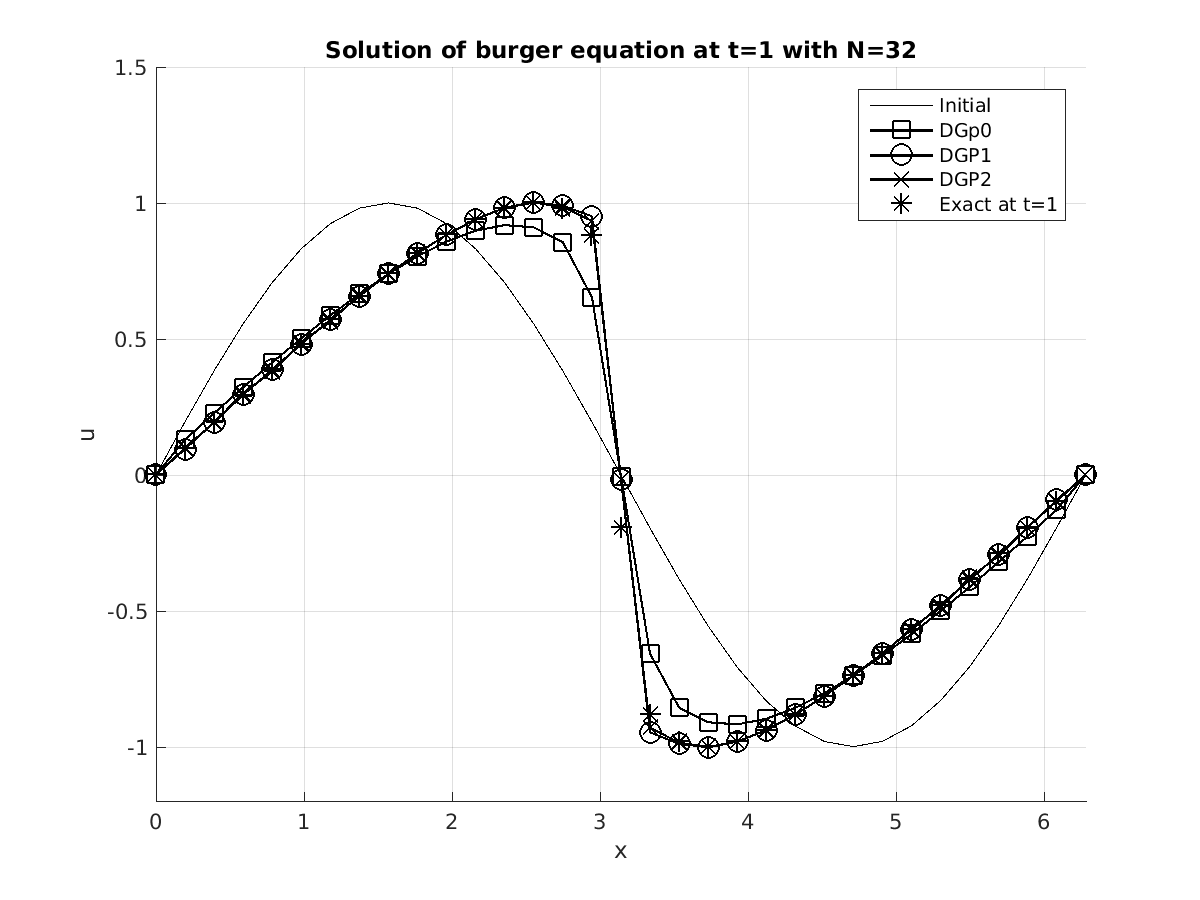
\includegraphics[width=0.8\linewidth]{1burger_sin_t_1}}
%
\subfigure[t=2]{%
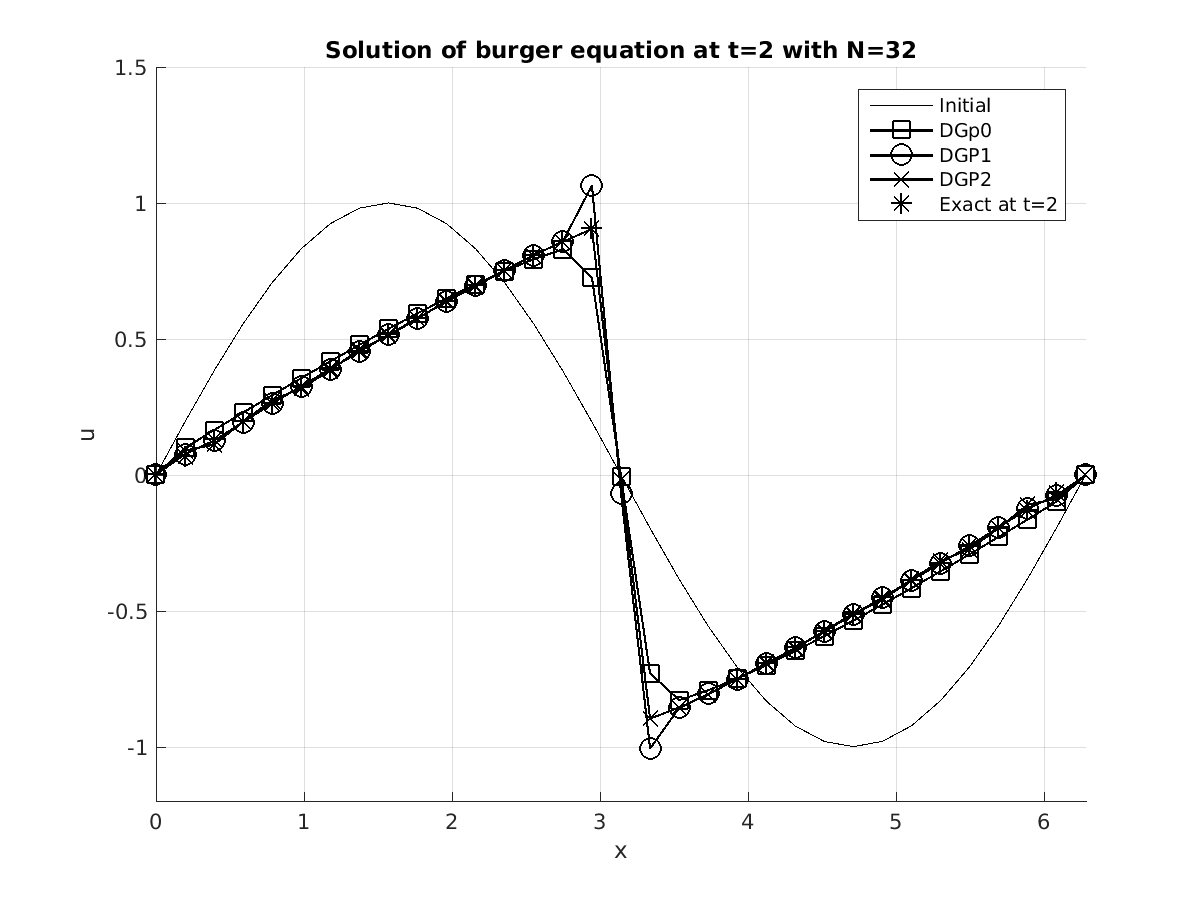
\includegraphics[width=0.8\linewidth]{2burger_sin_t_2}}
%
\caption{Comparison of numerical solution of burger equation with analytical solution for a sin wave.}
\label{sinwave}
\end{figure}

\begin{figure}[ht]
\centering
\subfigure[t=1]{%
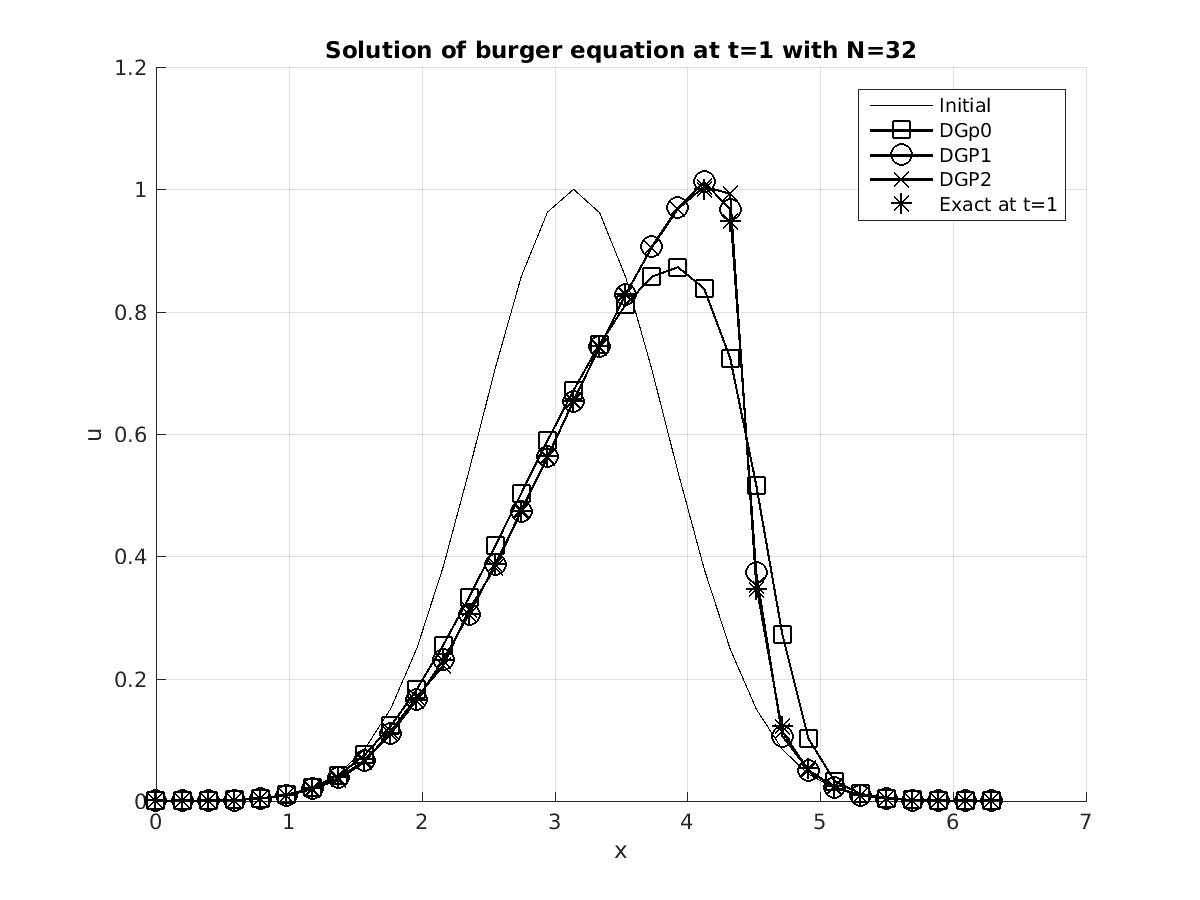
\includegraphics[width=0.8\linewidth]{3burger_bump_t_1}}
%
\subfigure[t=2]{%
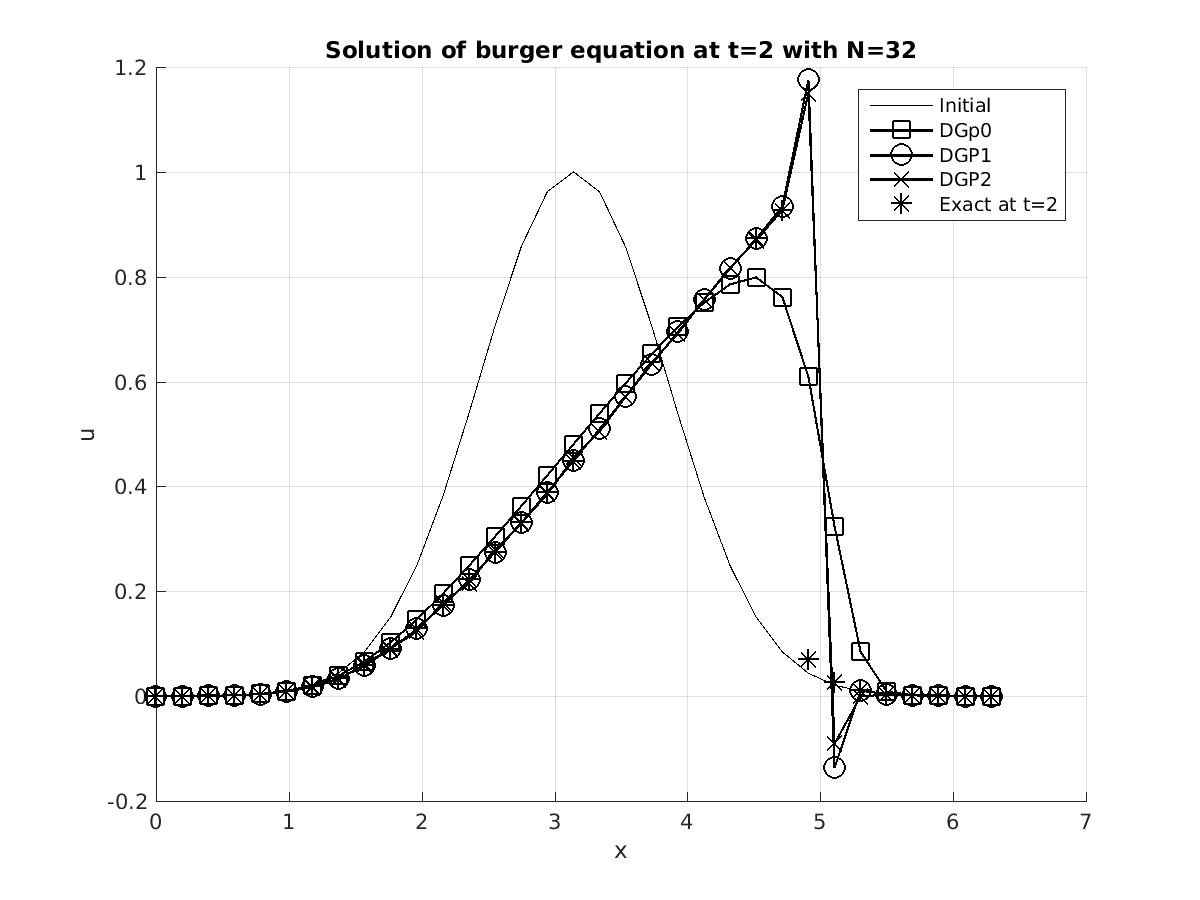
\includegraphics[width=0.8\linewidth]{4burger_bump_t_2}}
%
\caption{Comparison of numerical solution of burger equation with analytical solution for a Gaussian pulse.}
\label{gaussian}
\end{figure}

\clearpage
After successfully testing the DG methods for burger equation, the program is appended to include the discretization of diffusion terms. Two types of methods have been implemented to discretize the diffusion terms: BR2 and DDG. First, the order of accuracy of these methods is determined by solving just the diffusion equation(a=b=0 c=1) with an initial condition as $u(x,0)=sin(x)$ on a domain, extending from x=0 to x=$\pi$, with 4, 8 ,16 ,32 cells . The exact solution for this case is derived using separation of variables and is given by $e^{-ct} sin(x)$. The solution is computed at t=2 and the L2 norm error is determined for all the grids.  The order of accuracy is determined by the relation between L2 norm error and grid size given by:

\begin{equation}
\begin{gathered}
||E||_{L^2}=C*h^{\alpha}\\
log10(||E||_{L^2})={\alpha}*log10(h)+log10(C)\\
\end{gathered}
\end{equation}
here alpha determines the order of accuracy. Fig. \ref{errorfun} shows the plot of log10(L2norm) vs log10(havg) for DDG method and BR2 method. The results shows that the DDG method is second order accurate and order of accuracy for BR2 method is less than DDG.

\begin{figure}[ht]
\centering
\subfigure[Error function]{%
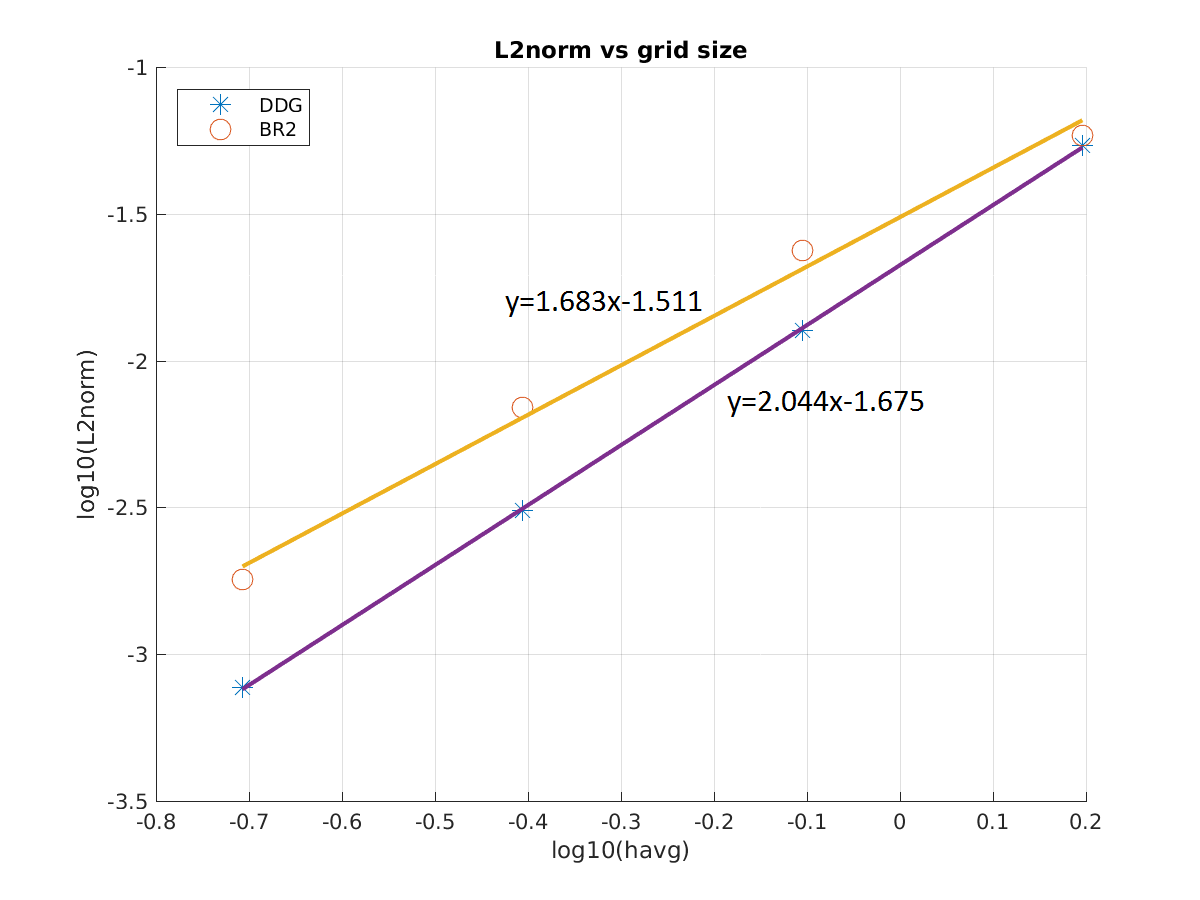
\includegraphics[width=0.8\linewidth]{5Errorfunction_diff_1d}}
%
\subfigure[Error function]{%
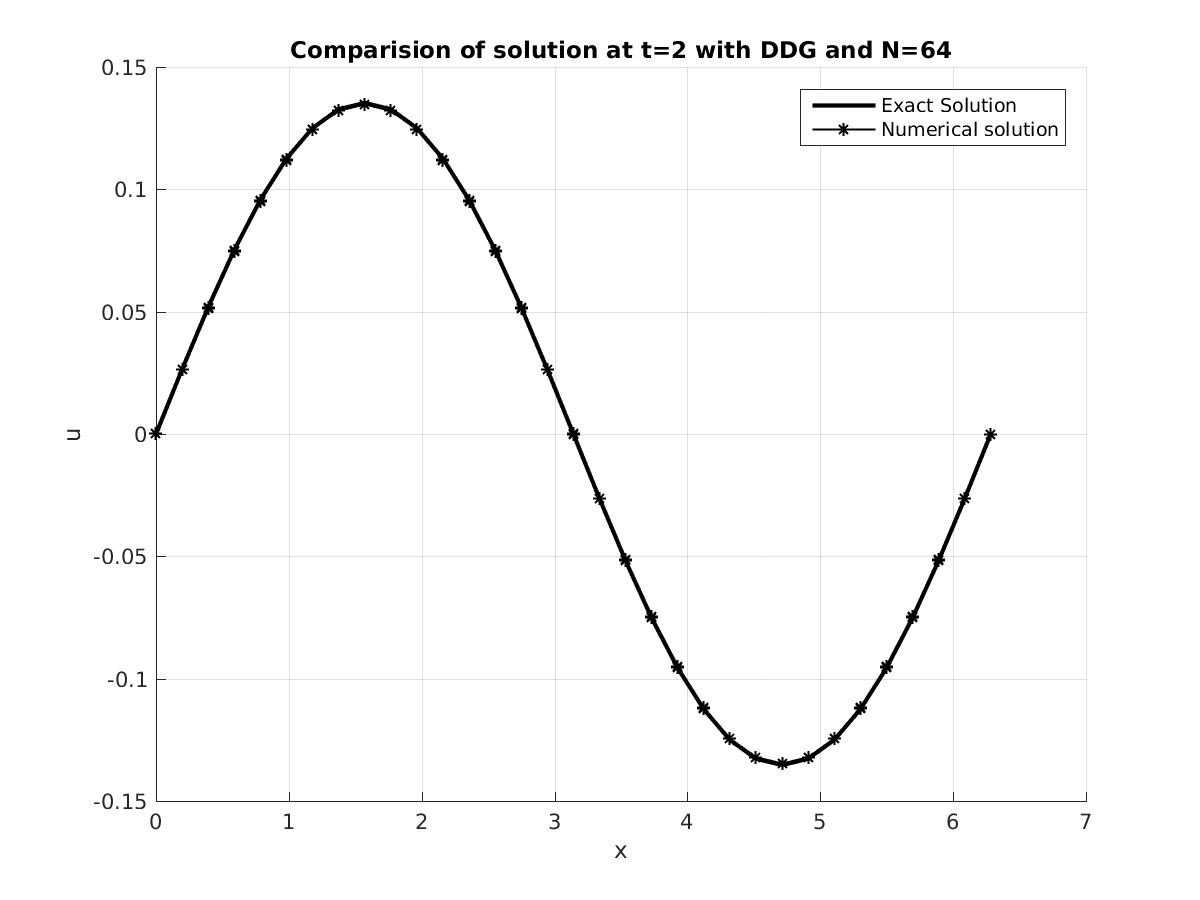
\includegraphics[width=0.8\linewidth]{6solution_ddg_t_2_diff}}
%
\caption{Solution of pure diffusion problem }
\label{errorfun}
\end{figure}

\clearpage

Next the code for entire nonlinear advection-diffusion equation is tested on a computations domain includes 4000 mesh cells extending form x=-10 to x=40 with a=1 b=1 c=1.5e-5 and following initial condition

\begin{equation}
\begin{gathered}
u(x,0)=u_0 exp((-\beta x)^10)sin(2pix)\\
u_0=7.96e-3 \quad \beta=0.179
\end{gathered}
\end{equation}

Fig. \ref{DDGsel} shows the solution at t=30 with DDG method and Fig \ref{BR2} shows the solution using BR2 method. It can be observed the sin wave distorts creating sharp gradients due to nonlinear advection and the wave is adverted with a velocity of 1 because of the linear advection term.

\begin{figure}[ht]
\centering
\subfigure[Solution]{%
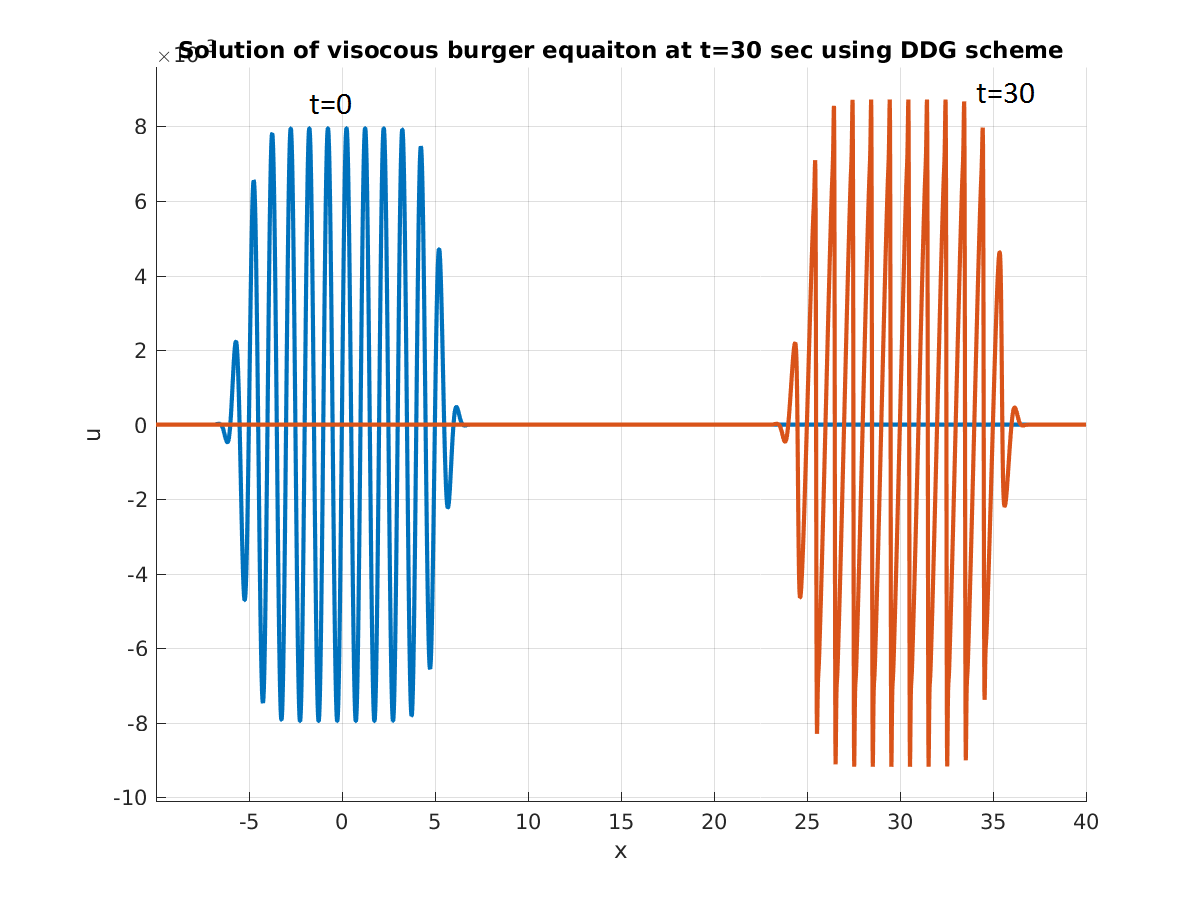
\includegraphics[width=\linewidth]{7solution_ddg_t_30_prob2}}
%
\subfigure[Solution]{%
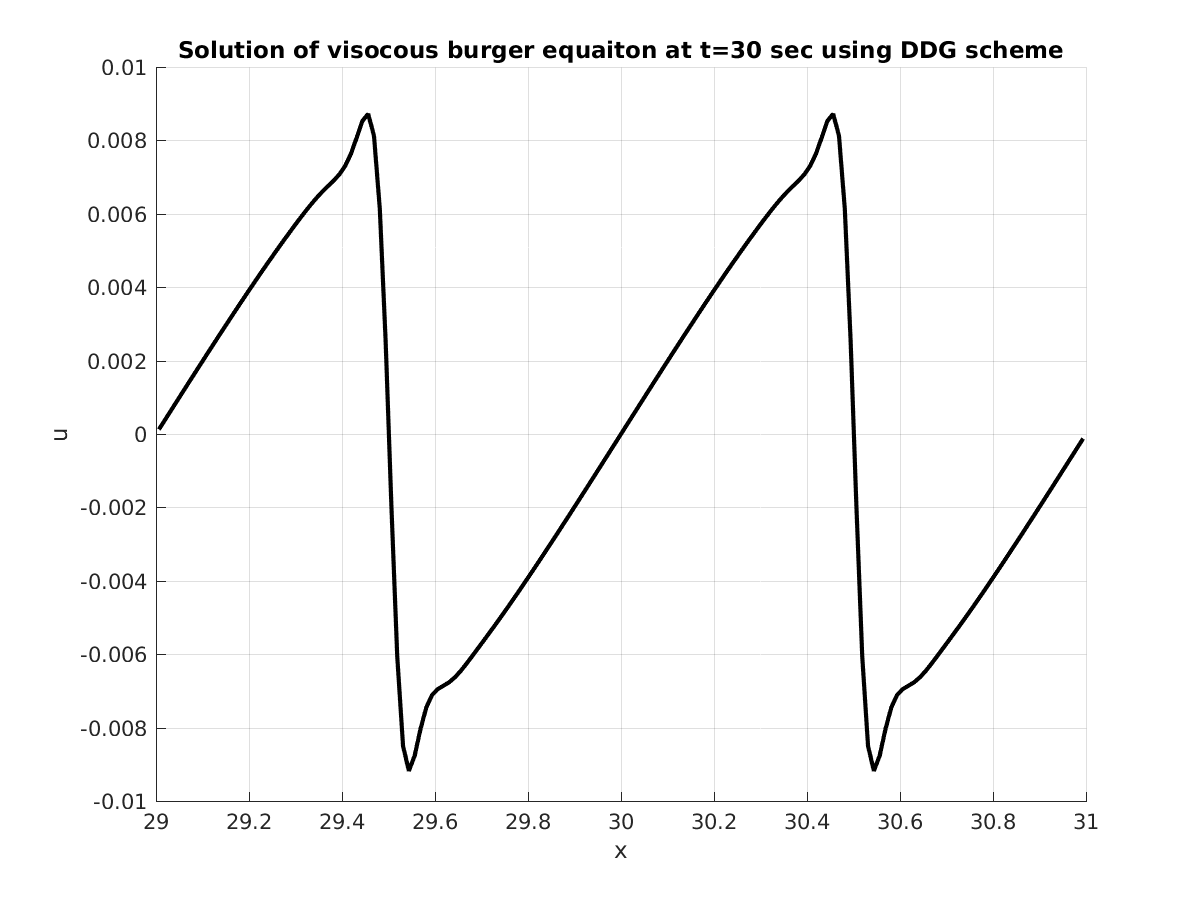
\includegraphics[width=1.0\linewidth]{8solution_ddg_t_30_prob2_2}}
%
\caption{Solution using DDG }
\label{DDGsel}
\end{figure}

\begin{figure}[ht]
\centering
\subfigure[Solution]{%
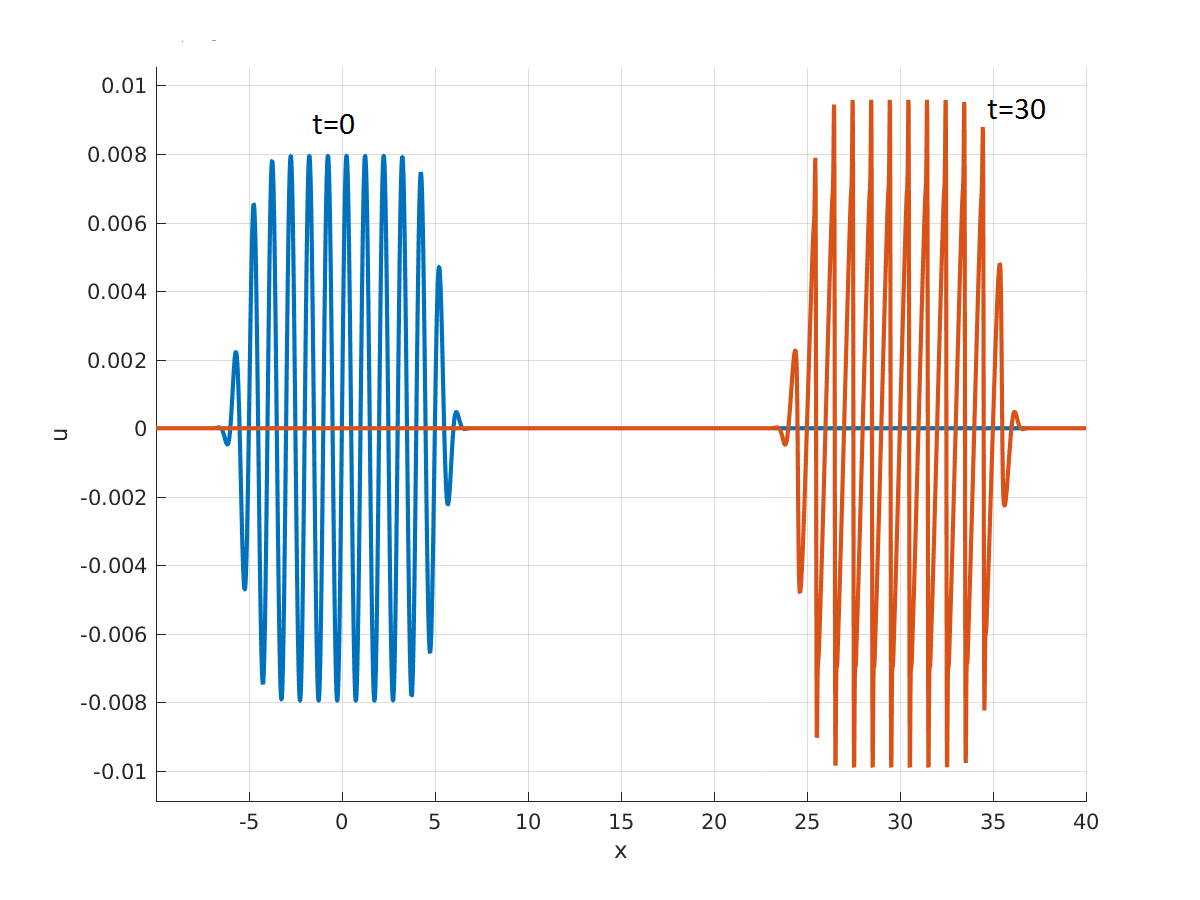
\includegraphics[width=0.8\linewidth]{9solution_ddg_t_30_prob2_br2}}
%
\subfigure[Solution]{%
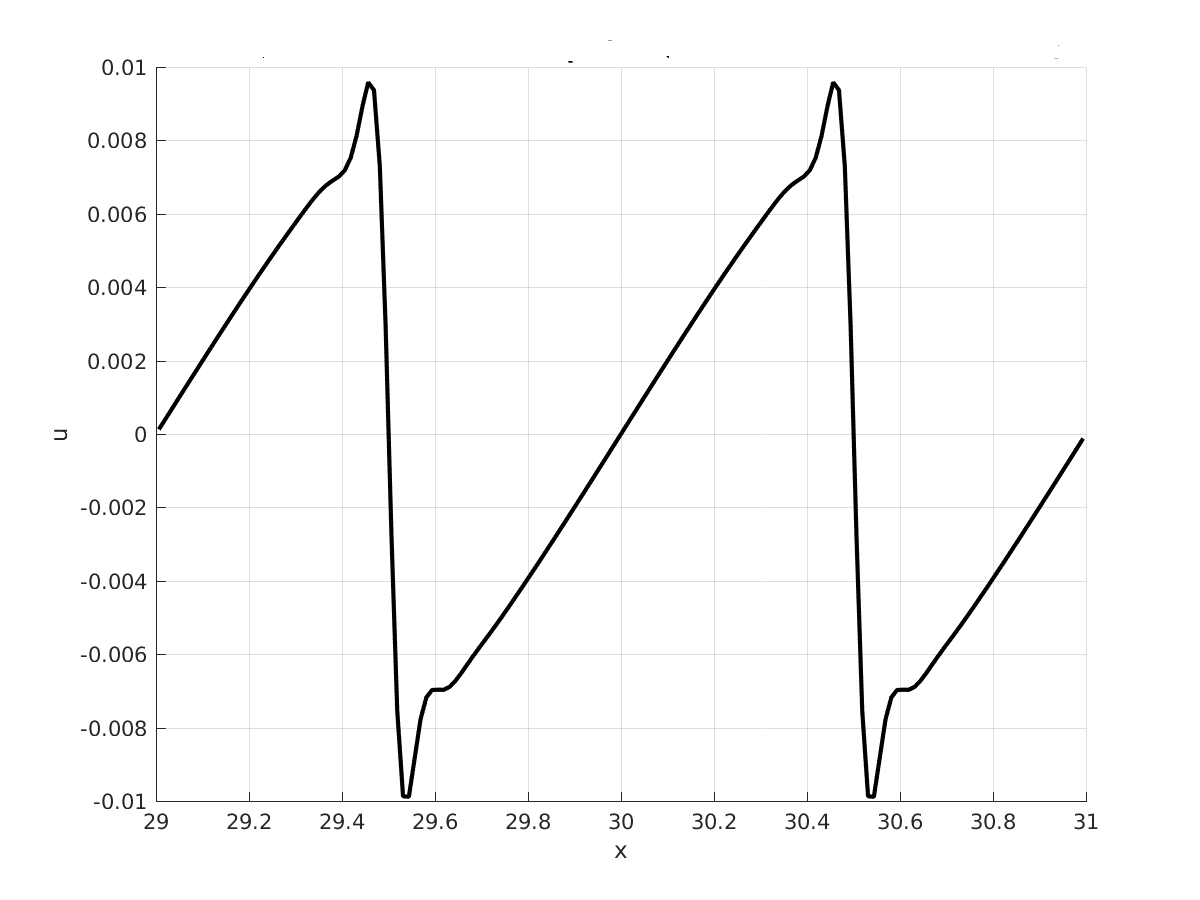
\includegraphics[width=0.8\linewidth]{10solution_ddg_t_30_prob2_2_br2}}
%
\caption{Solution using BR2 Method}
\label{BR2}
\end{figure}
\clearpage
\section{Conclusion}
The DG methods are tested successfully by solving diffusion equations using DDG and BR2 method. It is observed that the order of accuracy is second with both the methods. In conclusion DG methods will increase the order of accuracy if used for solving flow equations.



%% The Appendices part is started with the command \appendix;
%% appendix sections are then done as normal sections
%% \appendix

%% \section{}
%% \label{}

%% References
%%
%% Following citation commands can be used in the body text:
%% Usage of \cite is as follows:
%%   \cite{key}          ==>>  [#]
%%   \cite[chap. 2]{key} ==>>  [#, chap. 2]
%%   \citet{key}         ==>>  Author [#]

%% References with bibTeX database:

\bibliographystyle{model1-num-names}
\bibliography{sample.bib}

%% Authors are advised to submit their bibtex database files. They are
%% requested to list a bibtex style file in the manuscript if they do
%% not want to use model1-num-names.bst.

%% References without bibTeX database:

% \begin{thebibliography}{00}

%% \bibitem must have the following form:
%%   \bibitem{key}...
%%

% \bibitem{}

% \end{thebibliography}


\end{document}

%%
%% End of file `elsarticle-template-1-num.tex'.
